%!TEX root = main.tex

\chapter{Introduction}
\label{introduction}

% bla
\begin{figure}[h!]
	\centering
	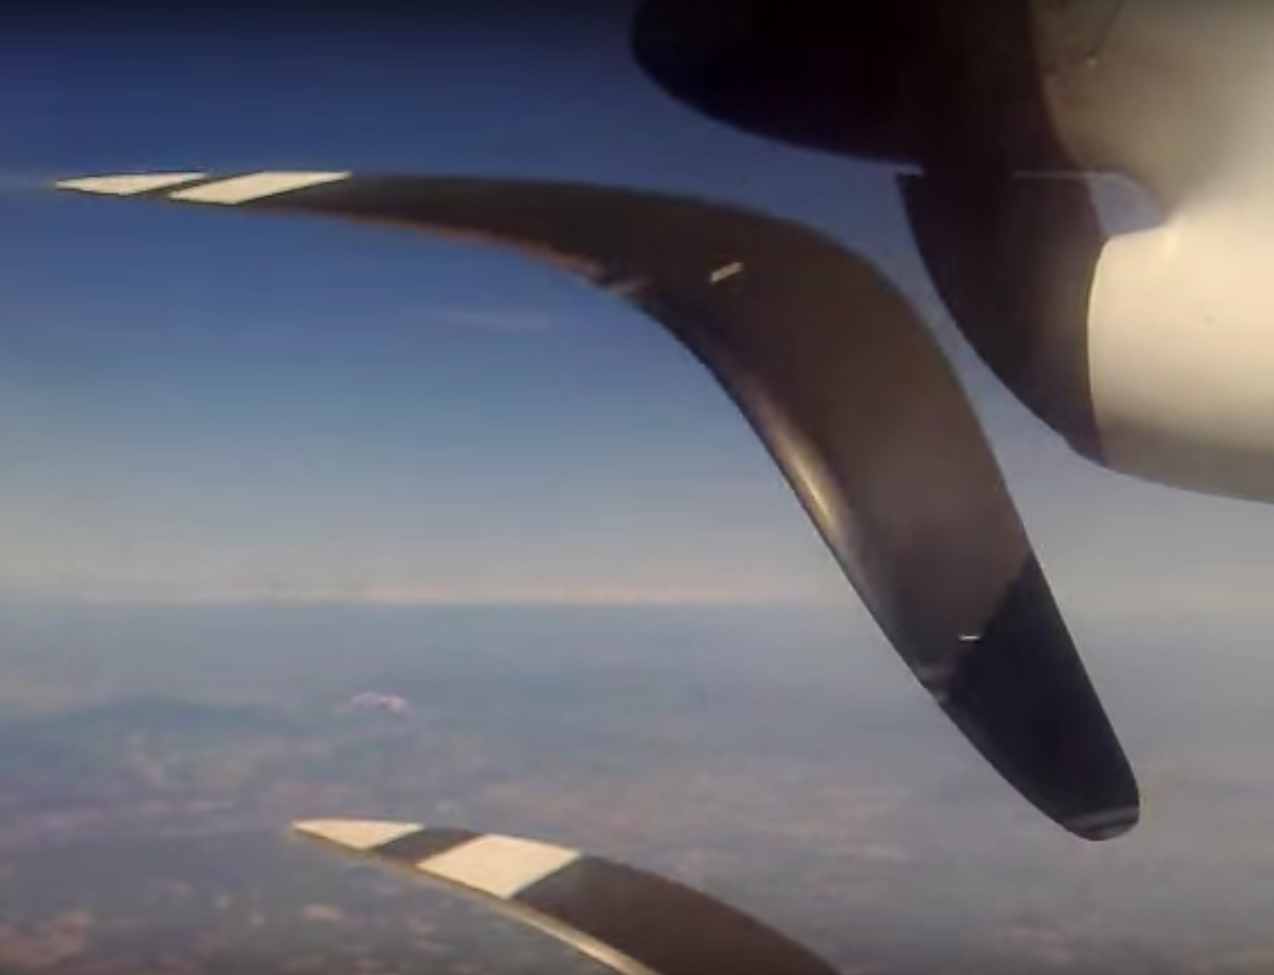
\includegraphics[width=\textwidth]{intro}
	\caption[shortCaption]
	{Weird effects of digital signals in video}
	\label{fig:label}
\end{figure}

\clearpage

This section tries to make sure we are all on the same page. It goes through some mathematics notation and principles of digital audio.\\
If you rather want a video format revision of digital audio (I mean, it's \the\year, of course you want), I can recommend \href{https://www.youtube.com/watch?v=cIQ9IXSUzuM}{D/A and A/D | Digital Show and Tell (Monty Montgomery @ xiph.org) }\footnote{https://www.youtube.com/watch?v=cIQ9IXSUzuM}. Some of the points in the video go beyond what we are doing here and vice versa, so don't purely rely on the video though. \\
Ideally, if you throughly understood the introduction section, you should be able to go through the remaining chapters with tempo.\\

\section{About this document}

Some information in this document is relevant for understanding it's contents but not relevant for the exam. For example in chapter \ref{Modulation} we will find a really complicated result of an equation. The point there is just that it's complicated. And it is shown how complicated, but this is nothing to be learned by heart.\\
Please report any mistakes, errors etc to \href{mailto:ptrk.lechner@gmail.com}{ptrk.lechner@gmail.com}.

\begin{mdframed}[backgroundcolor=black!10,rightline=false,leftline=false]
\textbf{Text and equations with a gray background like this are background information that is not to be learned by heart.}
\end{mdframed}

\begin{framed}

	\textbf{Video analogies}\\
	This document tries to explain digital signals. It does this by use of audio signal mainly. Sometimes video analogies are given. These are also not relevant for the exam.

\end{framed}


\section{About plotting signals}

We will need to plot a lot of signals in order to understand them better. Most of the time, such a plot will look like figure \ref{fig:simpeSine}.

\begin{figure}[h!]
	\centering
	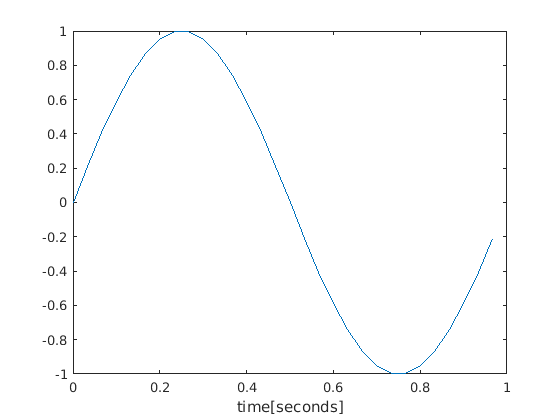
\includegraphics[width=11cm]{simpleSine}
	\caption[simple sine plot]
	{Sine wave, 1Hz, sampled at 30Hz sample rate}
	\label{fig:simpeSine}
\end{figure}

This plot looks nice but it has a problem. The sine wave is sampled at a sampling rate of 30 Hz, but we see a continuous line. This ``connection of the dots'' is created by plotting. It is kind of similar to what our \textit{digital-to-analog-converter} does. It somehow\footnote{linear interpolation in case of the plot} interpolates the values we have. \\
This can be misleading, so we should actually plot something more like figure \ref{fig:scatter}. Often we can see plots that look like figure \ref{fig:stem} as well when a signal is analyzed.

\begin{figure}[H]
	\centering
	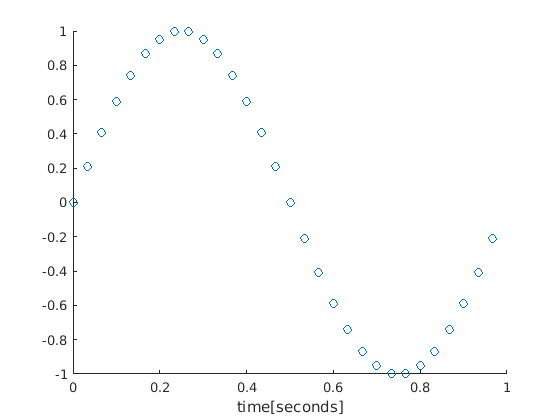
\includegraphics[width=11cm]{sineScatter}
	\caption[shortCaption]
	{Sine wave, 1Hz, sample rate 30Hz, scatter-plot}
	\label{fig:scatter}
\end{figure}



\begin{figure}[H]
	\centering
	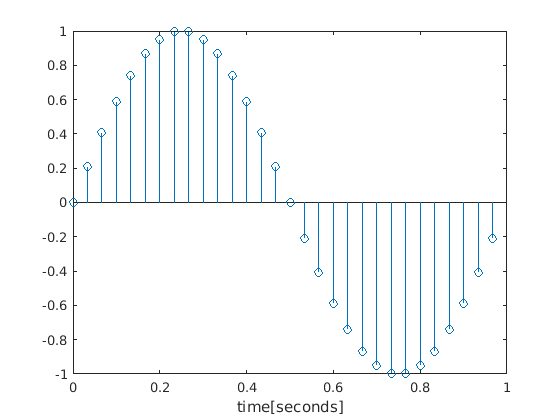
\includegraphics[width=11cm]{sineStem}
	\caption[shortCaption]
	{Sine wave, 1Hz, sample rate 30Hz, stem-plot}
	\label{fig:stem}
\end{figure}


So why don't we always do a stem- or scatter-plot? Simply because it gets too crowded with our usual sampling rates in audio. It just works with very low sampling rates or very short signals.\\
\begin{figure}[H]
	\centering
	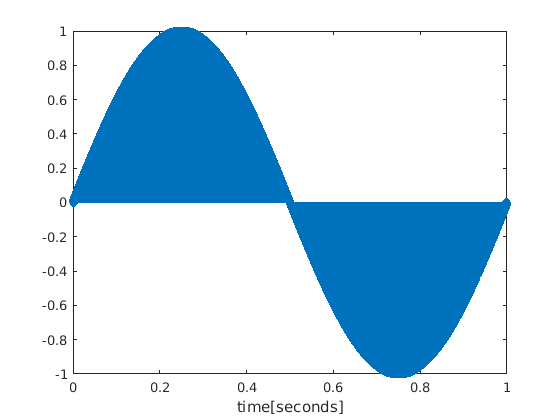
\includegraphics[width=11cm]{stem44100}
	\caption[shortCaption]
	{Sine wave, 1Hz, sample rate 44100Hz, stem-plot}
	\label{fig:label}
\end{figure}
\textbf{But we should never forget that we don't actually have the values in between the dots. Digital signals are not defined between their sampled points.}

\section{What is aliasing?}
Aliasing in audio means problems caused by signals that exceed the nyquist rate.\\
The nyquist rate,let's call it $f_n$ for now, is defined by the half of the sample rate ($f_s$). So, 
\begin{equation}
	f_n=\frac{f_s}{2}
\end{equation}
A digital system can only describe signals up to his nyquist rate. If we try to make signals higher than this frequency, we will fail and encounter strange effects.\\
Visually speaking, frequencies higher than nyquist fold back. So, let's assume we have a sampling rate of 100Hz. Nyquist would be at 50Hz. If we try to synthesize a sine wave with 51Hz, what we will get is a 49Hz one. If we try to make a 52Hz one, we will get 48Hz. So you see, it simply folds back.

\begin{framed}
	\textbf{Video analogies}\\
	Aliasing in graphics usually means \textit{spacial} aliasing, so aliasing in the space domain. This is what we see in figure \ref{fig:spAlias}. But there is also time domain aliasing in film. It is actually more natural to think about the sampling rate in audio as the same as the frame rate in video. For some really weird effects that arise in video due to time domain aliasing see \href{https://www.youtube.com/watch?v=LVwmtwZLG88}{airplane}\footnotemark , \href{https://www.youtube.com/watch?v=GBtHeR-hY9Y}{Water experiment}\footnotemark or \href{https://www.youtube.com/watch?v=jcOKTTnOIV8}{Guitar strings}\footnotemark .
	\begin{center}
		% \centering
		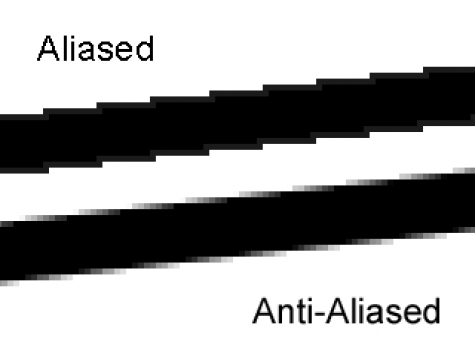
\includegraphics[width=7cm]{spacialAliasing1.png}
		\captionof{figure}{Spacial aliasing in graphics. The ``frequency'' of the intended pixels is to high for the actual pixels.}
		\label{fig:spAlias}
	\end{center}
	The particularly strange effects in the airplane example above are caused by the rolling shutter of a CMOS sensor. Since it is not sampling the incoming light uniformly (at the same time) the image is distorted.
\end{framed}
\footnotetext[2]{https://www.youtube.com/watch?v=LVwmtwZLG88}
\footnotetext[3]{https://www.youtube.com/watch?v=GBtHeR-hY9Y}
\footnotetext[4]{https://www.youtube.com/watch?v=jcOKTTnOIV8}

In fugure \ref{fig:cosAlias} you can see a visualization of aliasing in the time domain.  

\begin{figure}[H]
	\centering
	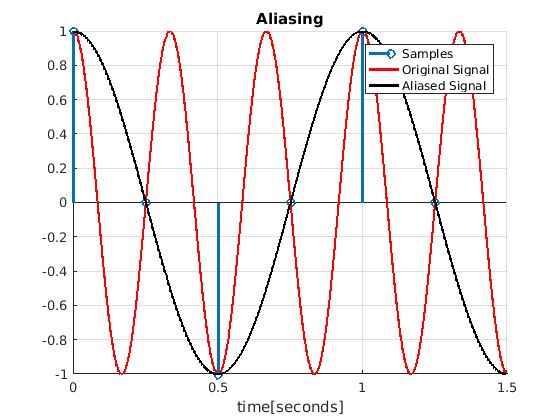
\includegraphics[width=\textwidth]{aliasingSine}
	\caption[shortCaption]
	{Aliasing visualized in the time domain. A sampling rate of 4 Hz is used. Therefore frequencies will fold above 2 Hz, which is the nyquist frequency. The input cosine has a frequency of 3 Hz, labeled ``Orginal Signal''. What we would get is the sampled points. If these are digital-to-analog converted, we would get what is labeled ``Aliased signal '' in this plot, so a 1 Hz cosine.}
	\label{fig:cosAlias}
\end{figure}



\section{Scaling and Mapping Signals}
It is an important skill to be able to scale signals from one range to another. We need it a lot and we will be able to think about signals more easily if we mastered this task. It's actually quite simple, we just have to imagine the signals visually.\\
So what exactly do we have to do here? We are confronted with the following problem: Given some signal, say, a sine wave with its maximum at the value 1 and its minimum at the value -1. How to bring it to a different range, say, 0-10?\\
It helps me a lot to solve this problem in two parts: first get the input in the range 0-1, then from there go to the desired range. What can we do to the signal? Let's take a sine wave:

\begin{figure}[h!]
	\centering
	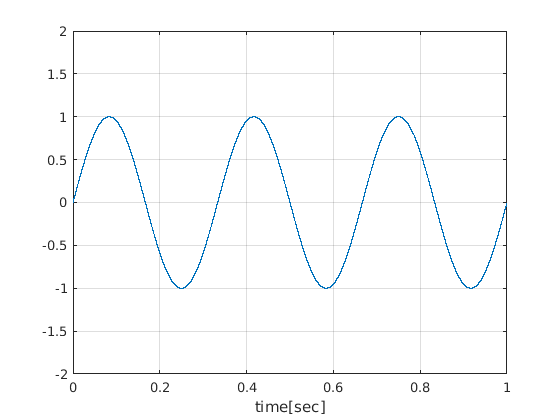
\includegraphics[width=11cm]{stdSine.png}
	\caption[a sine wave]
	{a sine wave}
	\label{fig:aSine}
\end{figure}
Well we can add and subtract to move the wave vertically, so let's add 1 to move it up:

\begin{figure}[h!]
	\centering
	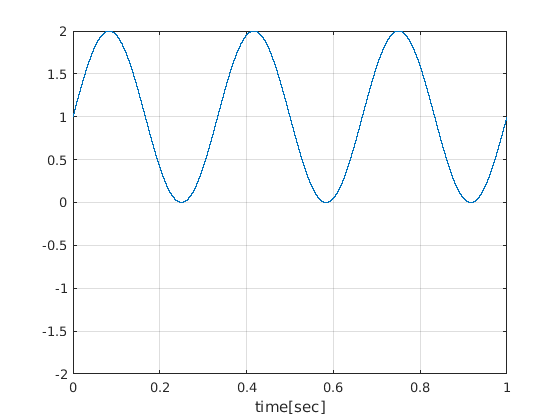
\includegraphics[width=11cm]{sinePlusOne.png}
	\caption[a sine wave]
	{the same sine wave, 1 added to a each sample, therefore shifted upwards.}
	\label{fig:aShiftedSine}
\end{figure}

So we can move signals around by adding constant values. We can scale them by multiplication. So if we take our sine that now ranges from 0 to 2 and multiply it by 0.5, we get whats in figure \ref{fig:sine01}.

\begin{figure}[h!]
 	\centering
 	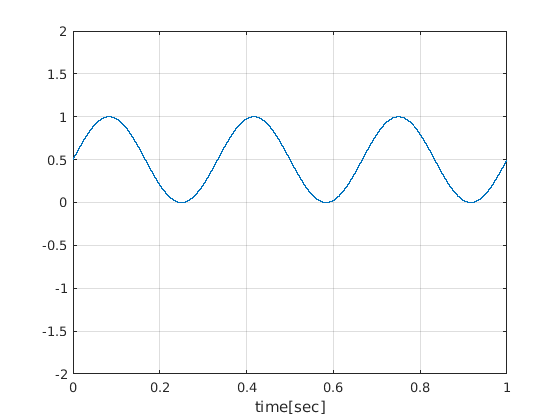
\includegraphics[width=11cm]{sine01.png}
 	\caption[sine 0 to 1]
 	{Sine with a range of 0-1. Obtained by taking a sine wave, adding 1 and dividing by two afterwards.}
 	\label{fig:sine01}
 \end{figure} 

Using what we got now in figure \ref{fig:sine01}, we can just multiply by 10, easy! Beware that there are always multiple solutions to this kind of a problem. Try to find another one for the problem above!

\begin{question}
Let's take a sine wave that has it's minimum at 2 and it's maximum at 5. What do we have to do to get it into a -1 to 1 range?
\end{question}
\begin{Answer}
We could subtract 1.5 to center the wave around zero first. Afterwards we take care of the amplitude by multiplying by $\frac{2}{3}$ (since the initial wave has a peak-to-peak amplitude of three and we want a peak-to-peak amplitude of 2)
\end{Answer}



\section{What's DC-Offset?}

What we did above by adding a constant value to a signal can be called adding DC-offset (``Gleichspannungsversatz''), DC-Bias or a DC component. These are different words for the same thing.\\
DC-offset can also be encountered in signals we recorded (caused by old or broken equipment mainly). But we have seen that we can also generate DC-offset.

\comm{work in progress.}


\section{What's an Impulse?}

\comm{work in progress.}


\section{How to describe audio mathematically}

If we want to talk about signals, or if we want to analyze them, it is often useful to look at the problem mathematically. First, let's introduce some conventions. They might look unfamiliar or complicated. But in fact it is not very complicated and knowing these conventions makes it easy to communicate (e.g. reading scientific papers about our topics or explaining something to another person).

\subsection{signals}

Usually we describe a \textit{digital} signal by a name, say $x$, (but you can call it however you want). If we want to talk about the individual samples, or values of the (mono) signal, we can use a subscript or parenthesis. So if the fith sample of $x$ is 1, we could write:
\begin{equation}
	x_5=1
\end{equation}
or 
\begin{equation}
	x(5)=1
\end{equation}
Oftentimes we like to talk about a signal more generally and we use $n$ as a place holder for this index, so we might write $x_n$, meaning the nth sample of $x$.

\subsubsection{sine waves}
We use sine waves a lot. The syntax can get a bit overwhelming at first, so let's quickly explain what's going on in a standard sine wave oscillator.
\begin{equation}
	x(t) = A \cdot sin(2\pi f t + \phi)
\end{equation}
Where $f$ is the frequency in Hertz and $t$ is the time in seconds. $\phi$ Is a (possibly constant) phase offset and $A$ can be used to scale the whole thing. Since cosine and sine have their peaks at -1 and 1, $A$ will be the amplitude. If $A$ is set to 0.5, the resulting signal will have it's peaks at -0.5 and 0.5.  
\comm{work in progress.}






\subsection{systems}

% \addsec{Was passiert in Epro und wofuer brauche ich es?}


\section{Message Domain/Signal Domain}

\comm{work in progress.}

